Aufgrund der hohen Popularität der $\lambda$-Architektur, gibt es Dienste, die sowohl Echtzeitverarbeitung, als auch Batch/\ac{OLAP}-Verarbeitung unterstützen.

\subsection{AWS IoT Analytics} \label{productselection:iotanalytics}



\AWSIOT Analytics ist ein Dienst der \AWSIOT Produktfamilie, der nach Aussage des Herstellers weitreichende Analysen von \ac{IoT} Daten, die beispielsweise via \AWSIOT Core geladen werden können, zulässt.\footcite[Vgl. auch im Folgenden][]{AmazonWebServicesInc..o.J.c} Dabei bietet der Dienst Lösungen für Sammlung, Verarbeitung, Speicherung, Analyse und Benachrichtigung/Visualisierung von Daten an, bzw. bietet Schnittstellen um diese Aufgaben zu erledigen. Im speziellen deckt \AWSIOT Analytics die Aufgaben einer $\lambda$-Architektur ab. So besitzt \AWSIOT Analytics beispielsweise eine integrierte Zeitreihendatenbank, welche ergänzend zu den Echtzeitdaten von \AWSIOT Core für Analysen genutzt werden kann.
\begin{figure}[H]
\centering
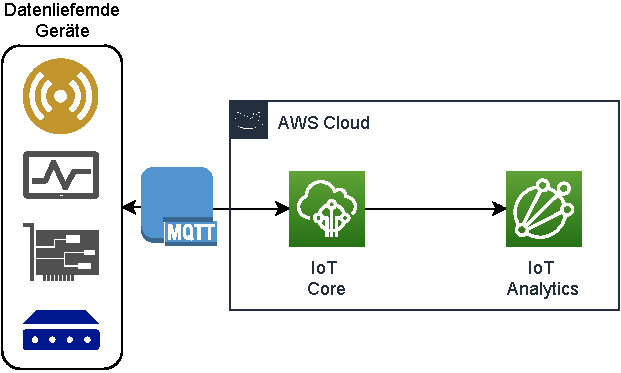
\includegraphics[width=0.8\textwidth]{graphics/IoT-Analytics-general.pdf}
\caption{Grobarchitektur des Ablaufes für IoT Analytics}
\label{abb:GrobArchitekturIoTAnalytics}
\end{figure}
In \autoref{abb:GrobArchitekturIoTAnalytics} ist die Grobarchitektur und Verknüpfung mit anderen Diensten unter Annahme der Vorraussetzungen aus \autoref{chap:rahmendatenverarbeitung} gezeigt. Datenliefernde Geräte, wie beispielsweise Sensoren liefern Zeitreihen-Messwerte via dem \ac{MQTT} Protokoll an. Die Weiterleitung zu IoT Analytics erfolgt mittels einer eingerichteten Regel im \ac{IoT} Core Messagebroker, welche mittels eines Dialekts der \ac{SQL} Sprache gewisse Topics vorselektiert oder alle Topics zulässt.

\Todo{Erklärung Analytics Compute Unit (Notebooks)}

\subsubsection{Featurevergleich}
Median und Quantile
Anomaliedetektion
Schwellwertüberschreitung
Trenderkennung/gleitender Durchschnitt



\subsubsection{Performancevergleich}
\Todo{Performancegarantien}

\subsubsection{Kostenvergleich}
\begin{table}[H]
\centering
\begin{tabular}{|l|l|l|}
\hline
Dimension & Preis(\$)/Einheit & Summe (\$) \\ \hline
Datenverarbeitung  & 0,20/GB & 1,728  \\\hline
Datenspeicherung verarbeitet  & 0,03/GB & 0,7776  \\\hline
Anfragenbearbeitung & \begin{tabular}[c]{@{}l@{}}6,5 \\ 0,00634/GB\end{tabular} & 157,95 \\ \hline
\begin{tabular}[c]{@{}l@{}}Datenspeicherung roh\\ \ac{S3}\\ Standard Tier\end{tabular}  & 0,0245/GB & 0,63504  \\\hline
Summe & \cellcolor[HTML]{EFEFEF} & \underline{161,09064}  \\\hline
%Eigene Analyselogik  & 0,36/h & x  \\\hline
\end{tabular}
\caption{Kostenvergleich AWS~IoT~Analytics}
\label{tab:kostenvergleich-AWS~IoT~Analytics}
\end{table}
In \autoref{tab:kostenvergleich-AWS~IoT~Analytics} sind die kalkulierten Preise nach gängiger Preismatrix dargestellt.\footcite[Vgl. auch im Folgenden][]{AmazonWebServicesInc..o.J.i} Das bestehende \enquote{Free Tier}, welches \ac{AWS} für den Dienst anbietet wird ignoriert, da es nur in den ersten zwölf Monaten der Nutzung des Dienstes verrechnet wird. Bei \ac{S3} wird angenommen, dass die Standard Speicherklasse verwendet wird und Volumenrabattierungen bei Datenvolumina >50TB im Monat nicht relevant sind.\footcite[Vgl. auch im Folgenden][]{AmazonWebServicesInc..o.J.j} Andere Speicherklassen sind günstiger, somit gibt die Schätzung eine Obergrenze für die \ac{S3} Preise.

\subsubsection{Gesamtbewertung}

\produktbewertung{AWS~IoT~Analytics}{8,10,7,7,7,5,5,4,2,1,0,57}
% In \autoref{tab:bewertungsmatrix-AWS~IoT~Analytics} wird AWS~IoT~Analytics gemäß der in \autoref{tab:einstufungen} eingeschränkten Bewertungen bewertet.

\subsection{Produktauswahl}
\begin{table}[H]
\centering
\begin{tabular}{|l|l|l|}
\hline
Platz & Name & Summe \\ \hline
1 & \AWSIOT Analytics & \cellcolor[HTML]{DAE8FC}57 \\ \hline
\end{tabular}
\caption{Produktreihenfolge Multimodus}
\label{tab:Reihenfolge-Multimodus}
\end{table}